% Version 1.2 of SN LaTeX, November 2022
%
% See section 11 of the User Manual for version history 
%
%%%%%%%%%%%%%%%%%%%%%%%%%%%%%%%%%%%%%%%%%%%%%%%%%%%%%%%%%%%%%%%%%%%%%%
%%                                                                 %%
%% Please do not use \input{...} to include other tex files.       %%
%% Submit your LaTeX manuscript as one .tex document.              %%
%%                                                                 %%
%% All additional figures and files should be attached             %%
%% separately and not embedded in the \TeX\ document itself.       %%
%%                                                                 %%
%%%%%%%%%%%%%%%%%%%%%%%%%%%%%%%%%%%%%%%%%%%%%%%%%%%%%%%%%%%%%%%%%%%%%

%%\documentclass[referee,sn-basic]{sn-jnl}% referee option is meant for double line spacing

%%=======================================================%%
%% to print line numbers in the margin use lineno option %%
%%=======================================================%%

%%\documentclass[lineno,sn-basic]{sn-jnl}% Basic Springer Nature Reference Style/Chemistry Reference Style

%%======================================================%%
%% to compile with pdflatex/xelatex use pdflatex option %%
%%======================================================%%

%%\documentclass[pdflatex,sn-basic]{sn-jnl}% Basic Springer Nature Reference Style/Chemistry Reference Style


%%Note: the following reference styles support Namedate and Numbered referencing. By default the style follows the most common style. To switch between the options you can add or remove “Numbered” in the optional parenthesis. 
%%The option is available for: sn-basic.bst, sn-vancouver.bst, sn-chicago.bst, sn-mathphys.bst. %  
 
%%\documentclass[sn-nature]{sn-jnl}% Style for submissions to Nature Portfolio journals
%%\documentclass[sn-basic]{sn-jnl}% Basic Springer Nature Reference Style/Chemistry Reference Style
\documentclass[sn-mathphys,Numbered]{sn-jnl}% Math and Physical Sciences Reference Style
%%\documentclass[sn-aps]{sn-jnl}% American Physical Society (APS) Reference Style
%%\documentclass[sn-vancouver,Numbered]{sn-jnl}% Vancouver Reference Style
%%\documentclass[sn-apa]{sn-jnl}% APA Reference Style 
%%\documentclass[sn-chicago]{sn-jnl}% Chicago-based Humanities Reference Style
%%\documentclass[default]{sn-jnl}% Default
%%\documentclass[default,iicol]{sn-jnl}% Default with double column layout

%%%% Standard Packages
\usepackage{graphicx}%
\usepackage{multirow}%
\usepackage{amsmath,amssymb,amsfonts}%
\usepackage{amsthm}%
\usepackage{mathrsfs}%
\usepackage[title]{appendix}%
\usepackage{xcolor}%
\usepackage{textcomp}%
\usepackage{manyfoot}%
\usepackage{booktabs}%
\usepackage{algorithm}%
\usepackage{algorithmicx}%
\usepackage{algpseudocode}%
\usepackage{listings}%
\usepackage{pythonhighlight}
%%%%

%%%%%=============================================================================%%%%
%%%%  Remarks: This template is provided to aid authors with the preparation
%%%%  of original research articles intended for submission to journals published 
%%%%  by Springer Nature. The guidance has been prepared in partnership with 
%%%%  production teams to conform to Springer Nature technical requirements. 
%%%%  Editorial and presentation requirements differ among journal portfolios and 
%%%%  research disciplines. You may find sections in this template are irrelevant 
%%%%  to your work and are empowered to omit any such section if allowed by the 
%%%%  journal you intend to submit to. The submission guidelines and policies 
%%%%  of the journal take precedence. A detailed User Manual is available in the 
%%%%  template package for technical guidance.
%%%%%=============================================================================%%%%

%\jyear{2021}%

%% as per the requirement new theorem styles can be included as shown below
\theoremstyle{thmstyleone}%
\newtheorem{theorem}{Theorem}%  meant for continuous numbers
%%\newtheorem{theorem}{Theorem}[section]% meant for sectionwise numbers
%% optional argument [theorem] produces theorem numbering sequence instead of independent numbers for Proposition
\newtheorem{proposition}[theorem]{Proposition}% 
%%\newtheorem{proposition}{Proposition}% to get separate numbers for theorem and proposition etc.

\theoremstyle{thmstyletwo}%
\newtheorem{example}{Example}%
\newtheorem{remark}{Remark}%

\theoremstyle{thmstylethree}%
\newtheorem{definition}{Definition}%

\raggedbottom
%%\unnumbered% uncomment this for unnumbered level heads

\begin{document}

\title[Manager Mauro]{Manager Mauro}

%%=============================================================%%
%% Prefix	-> \pfx{Dr}
%% GivenName	-> \fnm{Joergen W.}
%% Particle	-> \spfx{van der} -> surname prefix
%% FamilyName	-> \sur{Ploeg}
%% Suffix	-> \sfx{IV}
%% NatureName	-> \tanm{Poet Laureate} -> Title after name
%% Degrees	-> \dgr{MSc, PhD}
%% \author*[1,2]{\pfx{Dr} \fnm{Joergen W.} \spfx{van der} \sur{Ploeg} \sfx{IV} \tanm{Poet Laureate} 
%%                 \dgr{MSc, PhD}}\email{iauthor@gmail.com}
%%=============================================================%%

\author{\textbf{Lia Zerquera Ferrer},
\textbf{Daniel C\'ardenas Cabrera}}

%%==================================%%
%% sample for unstructured abstract %%
%%==================================%%



%%================================%%
%% Sample for structured abstract %%
%%================================%%

% \abstract{\textbf{Purpose:} The abstract serves both as a general introduction to the topic and as a brief, non-technical summary of the main results and their implications. The abstract must not include subheadings (unless expressly permitted in the journal's Instructions to Authors), equations or citations. As a guide the abstract should not exceed 200 words. Most journals do not set a hard limit however authors are advised to check the author instructions for the journal they are submitting to.
% 
% \textbf{Methods:} The abstract serves both as a general introduction to the topic and as a brief, non-technical summary of the main results and their implications. The abstract must not include subheadings (unless expressly permitted in the journal's Instructions to Authors), equations or citations. As a guide the abstract should not exceed 200 words. Most journals do not set a hard limit however authors are advised to check the author instructions for the journal they are submitting to.
% 
% \textbf{Results:} The abstract serves both as a general introduction to the topic and as a brief, non-technical summary of the main results and their implications. The abstract must not include subheadings (unless expressly permitted in the journal's Instructions to Authors), equations or citations. As a guide the abstract should not exceed 200 words. Most journals do not set a hard limit however authors are advised to check the author instructions for the journal they are submitting to.
% 
% \textbf{Conclusion:} The abstract serves both as a general introduction to the topic and as a brief, non-technical summary of the main results and their implications. The abstract must not include subheadings (unless expressly permitted in the journal's Instructions to Authors), equations or citations. As a guide the abstract should not exceed 200 words. Most journals do not set a hard limit however authors are advised to check the author instructions for the journal they are submitting to.}



%%\pacs[JEL Classification]{D8, H51}

%%\pacs[MSC Classification]{35A01, 65L10, 65L12, 65L20, 65L70}

\maketitle

\section{Descripci\'on del problema}\label{sec1}

\begin{center}
    Manager Mauro
\end{center} 

Mauro tiene un espíritu deportivo tan grande, que paralelamente con sus estudios ha decidido también manejar el equipo de fútbol de su facultad MATCOM. Dedicar su tiempo a esto no es impedimento (cree él) para seguir obteniendo buenos resultados académicos. La verdad sea dicha, Mauro no tiene ni idea de fútbol. De hecho, varias veces se ha preguntado a sí mismo cómo llegó a esa importante posición. Lo bueno es que sí sabe de matemática y porgramación, así que decide formar un equipo (teóricamente) poderoso. Mejor aún, el equipo más (teóricamente) poderoso posible.\\

Se debe formar un equipo de \textit{p}
 jugadores en distintas posiciones y \textit{k}
 espectadores VIP (comisión de embullo). La facultad tiene \textit{n} 
 personas. Para cada persona \textit{i}
 se conoce su valor $ a_i$
 como espectador VIP y su valor $p_{ij}$
 como jugador en la posición \textit{j}
.\\

Ayude a Mauro haciendo un algoritmo que calcule el poder (valor) del mejor equipo posible. Un equipo es mejor que otro si tiene más valor.

\section{Inputs y Outputs }\label{sec2}

Nuestro problema tiene tres entradas:
\begin{itemize}
    \item \textbf{n} representa la cantidad de personas 
    \item \textbf{A} lista de tama\~no n donde el valor de la pocisi\'on \textit{i} es el valor de la persona $a_i$ como espectador
    \item \textbf{V} matriz de tama\~no mxn donde m son posiciones que pueden ocupar los jugadores y la posici\'on $p_{ij}$ es el valor de del jugador i en la posici\'on j
    \item \textbf{p} representa la cantidad de jugadores que deben conformar al equipo
    \item \textbf{k} representa la cantidad de espectadores que deben asistir
\end{itemize}\\
Lo que se quiere devolver es lo siguiente :
 \begin{itemize}
     \item \textbf{v} que represente el valor del mejor equipo posible.
     \item \textbf{P} matriz de los jugadores que van a jugar y sus respectivas posiciones 
     \item \textbf{K} lista de jugadores que van a formar parte del p\'ublico
 \end{itemize}

\section{Primer Acercamiento}\label{sec4}
Una primera idea para resolver este problema es probar todas las posibles combinaciones de p jugadores y k espectadores. Luego de este nos quedamos con la combinación que maximice el valor del equipo, retornamos el valor del equipo, los jugadores con sus respectivas posiciones y los espectadores.
\subsection*{Análisis y formalización  del primer acercamiento}
La primera parte de este acercamiento consiste en buscar las posibles combinaciones\\
 Note que la cantidad de combinaciones de p jugadores y k espectadores en un conjunto n esta representada por la siguiente f\'ormula\\
 $$ C = \frac{n!}{p!(n-p)!} * \frac{(n-p)!}{k!(n-p-k)!}$$
\subsection*{Detalles de la implementaci\'on}
Para modelar nuestra soluci\'on con backtrack le a\~nadimos a la matriz V de entrada el vector A como una nueva columna,de esta manera obtenemos una matriz de m+1*n donde la \'ultima fila representa la posición espectador. \\

Se implement\'o una clase Team que representa la configuraci\'on del equipo que se va construyendo a medida que se van probando las combinaciones de jugadores.\\
 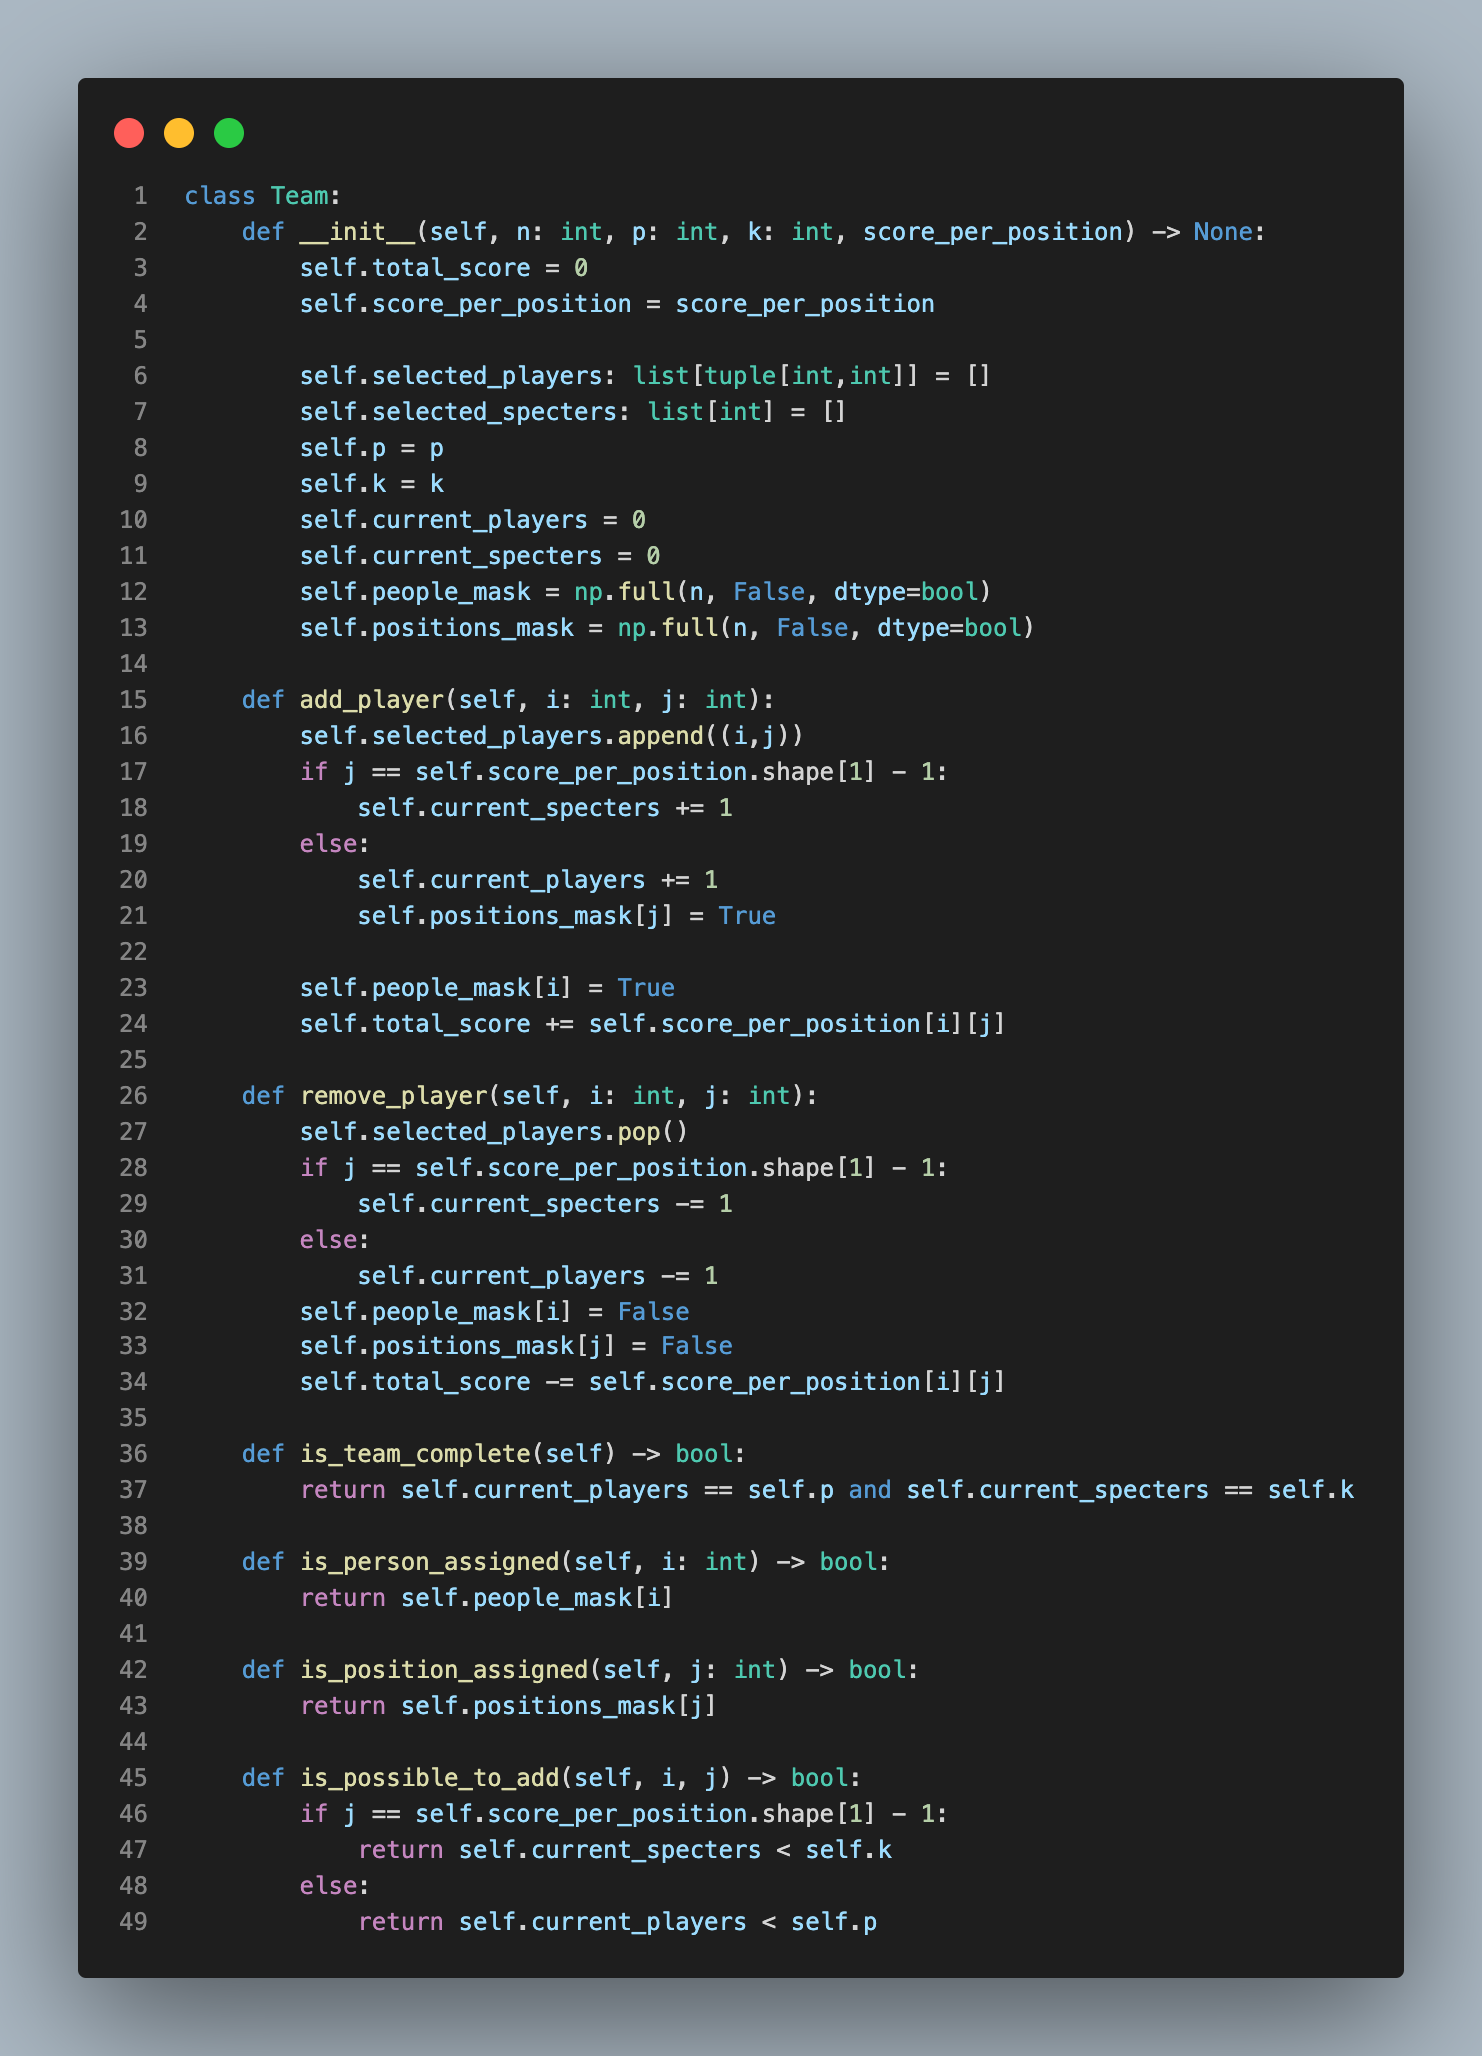
\includegraphics[width=0.8\textwidth]{code1.png}
\\
El m\'etodo \_brute\_force es el que se encarga de hacer el backtracking, cada vez que se a\~nade un jugador a la configuraci\'on de equipo, se hace un llamado recursivo con esa modificaci\'on, y as\'i sucede hasta que se pueda a\~nadir a mas jugadores, luego se quita el ultimo jugador puesto y se prueba con otro.
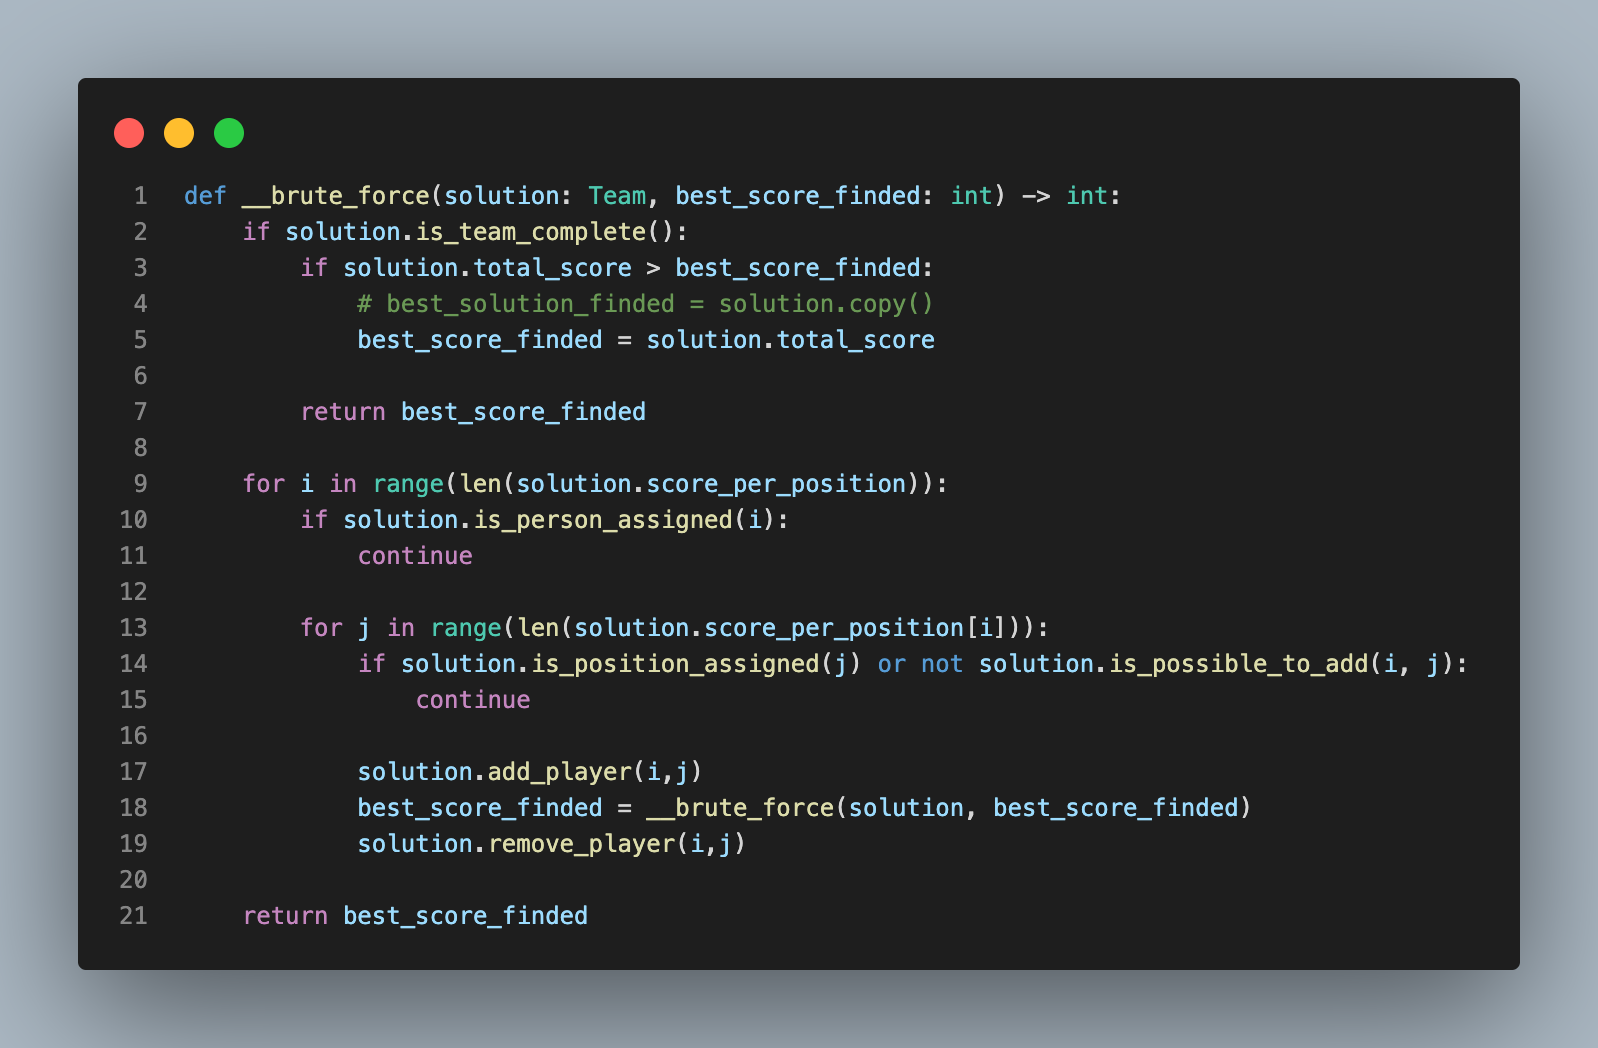
\includegraphics[width=0.8\textwidth]{code2.png}\\

La complejidad temporal es $O(n!)$ ya que se prueban todas las combinaciones\\
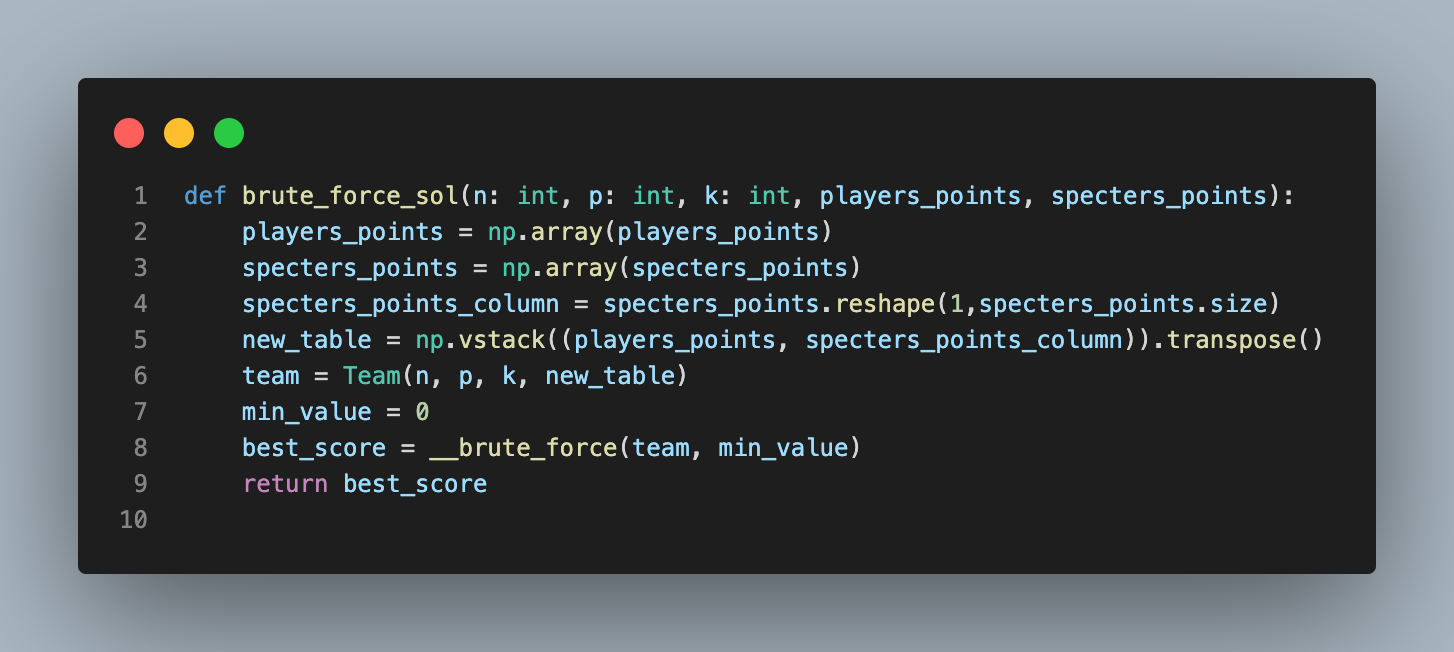
\includegraphics[width=0.8\textwidth]{code3.png}
\section{¿ C\'omo atacar este problema de combinatoria sin probar todas las combinaciones? }\label{sec4}
Nuestro objetivo es encontrar de un conjunto de n personas un subconjunto p de jugadores y y subconjunto k de espectadores de forma tal que la sumatoria de su valores como jugador y espectador respectivamente sea el valor máximo.\\ 
Como mencionamos en el primer acercamiento los espectador puede ser visto como posiciones dentro del equipo, debido a que se tienen que seleccionar k espectadores esto implicaría que se a\~naden k posiciones nuevas al equipo, representemos esto en una matriz.\\
Hasta el momento tenemos una matriz donde las columnas son los jugadores y de la fila 0 a la p se representan los posiciones de los jugadores y de la fila p+1 a la \'ultima(k filas) representan la posición espectador, note que p + k no necesariamente suman n, es decir que del conjunto de las n personas hay un subconjunto que no va a estar ocupando ninguna posición.\\
Observemos que no hacer nada también puede ser una posición del equipo es decir es rol que puede asumir un subconjunto de personas, por tanto si a\~nadimos n - (p+k) filas a la matriz con 0 en todas las posiciones de dichas filas(estas personas no aportan valor). Entonces el problema puede ser visto como un problema de asignaci\'on donde a cada persona de la facultad se le asigna un rol (jugador, espectador, no hacer nada) en una posici\'on espec\'ifica.\\

Representemos lo planteado anteriormente en la siguiente tabla:
\begin{table}[t]
\begin{center}
\begin{tabular}{| c | c | c | c | c | c | }
\hline
Roles & $n_1$  & $n_2$ & $n_3$ & ... & $n_n$ \\ \hline
$p_1$ &  $p_{1,1}$ &  $p_{1,2}$ &  $p_{1,3}$ &... &  $p_{1,4}$ \\ \hline
. & . & . & .& .& . \\ \hline
. & . & . & .& .& .\\ \hline
$p_p$ &  $p_{p,1}$ &  $p_{p,2}$ &  $p_{p,3}$ &... &  $p_{p,4}$\\ \hline
$k_1$ &  $k_{1,1}$ &  $k_{1,2}$ &  $k_{1,3}$ &... &  $k_{1,4}$\\ \hline
. & . & . & .& . & .\\ \hline
. & . & . & .& .& .\\ \hline
$k_k$ &  $k_{k,1}$ &  $k_{k,2}$ &  $k_{k,3}$ &... &  $k_{k,4}$\\ \hline
$r_1$ &  $r_{1,1}$ &  $r_{1,2}$ &  $r_{1,3}$ & ... &  $r_{1,4}$\\ \hline
. & . & . & .& .& .\\ \hline
. & . & . & .& .& .\\ \hline
$r_r$ &  $r_{r,1}$ &  $r_{r,2}$ &  $r_{r,3}$ &... &  $r_{r,4}$\\ \hline
\end{tabular}
\caption{Tabla donde cada fila es una posición y cada columna es una persona }
\label{tab:coches}
\end{center}
\end{table}\\
Notemos que cada persona solo puede ocupar una posición a la vez y la misma posición no puede estar ocupada por m\'as de una persona.\\
En otras palabras si nos apoyamos de la \textbf{Tabla 1} podemos decir que tomamos el valor de la posición  i y el  jugador  j, no podemos tomar mas ningún valor de la fila i ni de la columna j.\\
La \textbf{Tabla 1} puede ser vista como una matriz y dicha matriz nos puede dar la representación de un grafo G por matriz de adyacencia, donde cada persona va a tener aristas hacia todos los roles que puede tomar y la posición [i,j] representa el peso de la arista que asigna el rol i a la persona j.\\
Notemos que G es un grafo bipartito donde tenemos el conjuntos de personas(L) y el conjunto de roles(R).\\
Adem\'as podemos afirmar que el grafo G es bipartito completo ya que todas las $l \in L$(personas) tienen aristas hacia todas la $r \in R$(roles).\\
\subsection*{Modelando el problema con un grafo bipartito completo y ponderado}
Llegado a este punto tenemos nuestro problema modelado como un grafo G bipartito completo y ponderado, donde el objetivo es encontrar un emparejamiento  perfecto $M^*$ cuyas aristas tengan el máximo peso total sobre todos los emparejamiento perfectos.\\
Dicho de otra manera :\\
Sea $w(M) = \sum_{(l,r) in M} w(l,r)$ denotando el peso total sobre todos los emparejamientos perfectos, queremos encontrar $M^*$ tal que :
\begin{equation}
     w(M^*) = max\{w(M) : M ~es~emparejamiento~perfecto\} 
\end{equation}

\subsection{Algoritmo Húngaro}
El algoritmo Húngaro\cite{1} es conocido por resolver problemas de asignaci\'on en grafos bipartitos completos y ponderamos.\\
Dicho algoritmo recibe como parámetro de entrada un grafo G(V,E) bipartito completo y ponderado a partir del cual construye un subgrafo de igualdad $G_h$ tal que si en $G_h$ existe un emparejamiento perfecto $M^*$ entonces $M^*$ es la solución óptima del problema de asignación\footnote{\textbf{Theorema 25.14} Let G = (V,E), where V = LU R, be a complete bipartite graph where each adge (l,r) $\in$ E has weight w(l,r). Let h be a feasible vetex labeling of G and $G_h$  be the equality subgraph of G. If $G_h$ contains a perfect matching $M^*$, then $M^*$ is an optimal solution to the assingnment problme on G \cite{2}}.\\ 
Definamos el subgrafo $G_h$ de igualdad\\
Dado un etiquetamiento factible h, $G_h = (V,E_h)$ donde $G_h$ posee los mismos v\'ertices de G y el subconjunto de aristas $E_h = \{(l,r) \in E : l.h + r.h = w(l,r)\}$, donde h, etiquetamiento factible de la siguiente manera:\\
h es un etiquetamiento factible de G si $$l.h + r.h >= w(l,r)$$
\section{¿ C\'omo funciona el algoritmo Húngaro }
El algoritmo Húngaro comienza con un etiquetamiento factible cualquiera h y un emparejamiento $M^*$ en el subgrafo de igualdad $G_h$ y repetidamente busca camido M-aumentativos P en el $G_h$ y actualiza los emparejamiento con los caminos aumentativos P, logrando incrementar el tama\~no de los emparejamiento hasta conseguir en emparejamiento perfecto.
\begin{enumerate}
    \item ¿como obtener un etiquetamiento factible inicial?\\
    Respuesta: Siempre existe un etiquetamiento factible, ya que podemos tomar el etiquetamiento por defecto dado por:
    $$l.h = max \{ w(l,r) : r \in R\} ~ \forall ~l \in L$$
    $$r.h = 0 ~\forall ~r \in R$$
    \item ¿com\'o obtener el emparejamiento inicial? \\
    Respuesta: Se puede utiliza cualquier emparejamiento inicial, para desarrollar esta solución usamos particularmente el retornado por el algoritmo Greedy-Bipartite-Matching\cite{3}
    \begin{figure}[htb]
        \centering
        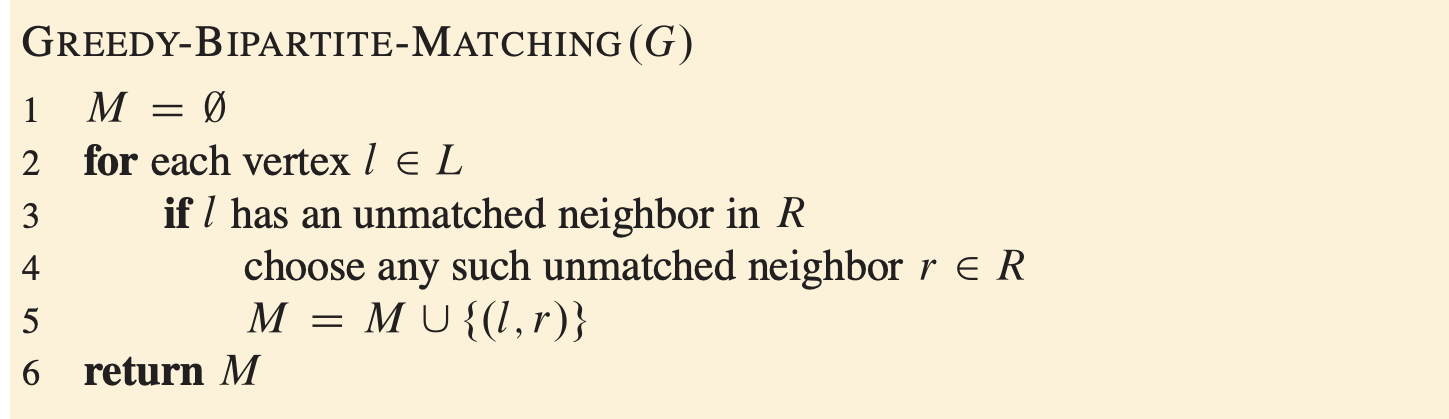
\includegraphics[width=0.8\textwidth]{Screenshot 2023-04-01 at 11.32.25 PM.png}
        \centering
        \caption{Greedy-Bipartite-Matching\cite{3}}
    \end{figure}\\
    Usamos este algoritmo porque el Greedy-Bipartite-matching devuelve un emparejamiento tal que su tamaño es al menos la mitad del emparejamiento m\'aximo.\\
    Probemos el anterior planteamiento: \\
    Sea $M^*$ un emparejamiento máximo y M el emparejamiento obtenido al aplicar Greedy-Bipartite-Matching.\\
    Sea \textbf{e} $\in$ M y \textbf{e} $\notin$ $M^*$\\
    Si agregamos la arista \textbf{e} al emparejamiento máximo, para que siga siendo un emparejamiento tendríamos que remover a los sumo dos aristas (las que que incidan sobre los vértices extremos de e).\footnote{Note que si agregamos esta nueva arista e a $M^*$ y no queda ningún vértice emparejado por mas de una arista tendríamos una contradicción porque entonces $M^*$ no seria máximo}.\\
    Luego si hacemos esto con todas las arista e tal que \textbf{e} $\in$ M y \textbf{e} $\notin$ $M^*$ obtenemos lo siguiente:\\
    \[
    \sum_{e^{'}\in M^*} 2e^{'} \geq \sum_{e\in M} e
    \]
    
    \[
    \sum_{e^{'}\in M^*} e^{'} \geq \frac{1}{2}\sum_{e\in M}
    \]
    \item ¿Com\'o encontrar en caso de que existan los caminos M-aumentativos en $G_h$? \\
    Respuesta : Para ello el algoritmo  crea un subgrafo de igualdad dirigido denotémoslo $G_{M,h}$ a partir de $G_h$\\
    $G_{M,h} = (V,E_{M,h})$ donde:
    \begin{equation}
         E_{M,h} = \{(l,r) : l \in L , r \in R~and~ (l,r) \in E_h - M \}~\cup ~\{(r,l) :l \in L , r \in R~and~ (l,r) \in M \}
    \end{equation}
   
    Nota: Se puede pensar en un camino M-aumentativo como un camino empezando desde un vértice no cubierto en L y terminando en un vértice no cubierto en R.\\
    ¿Com\'o se construye el camino M-aumentativo ?
    Para ello se hace una búsqueda desde cualquiera de los vértices de L no emparejados por M, hasta cualquiera de los vértices de R no emparejados por M haciendo una búsqueda en el grafo.\\
    Para empezar desde todos los vértices de L no emparejados inicializamos la cola con todos los vértices no  emparejados en L, en lugar de un solo vértice origen, luego al realizar el breadth search a partir de cada vértice de la cola se obtiene en bosque $F = (V_f,E_F)$ donde las raíces son los nodos no emparejados de L. Se puede observar el pseudocódigo de este algoritmo en la \textbf{Fig 2}.
    
    \begin{figure}[htb]
        \centering
        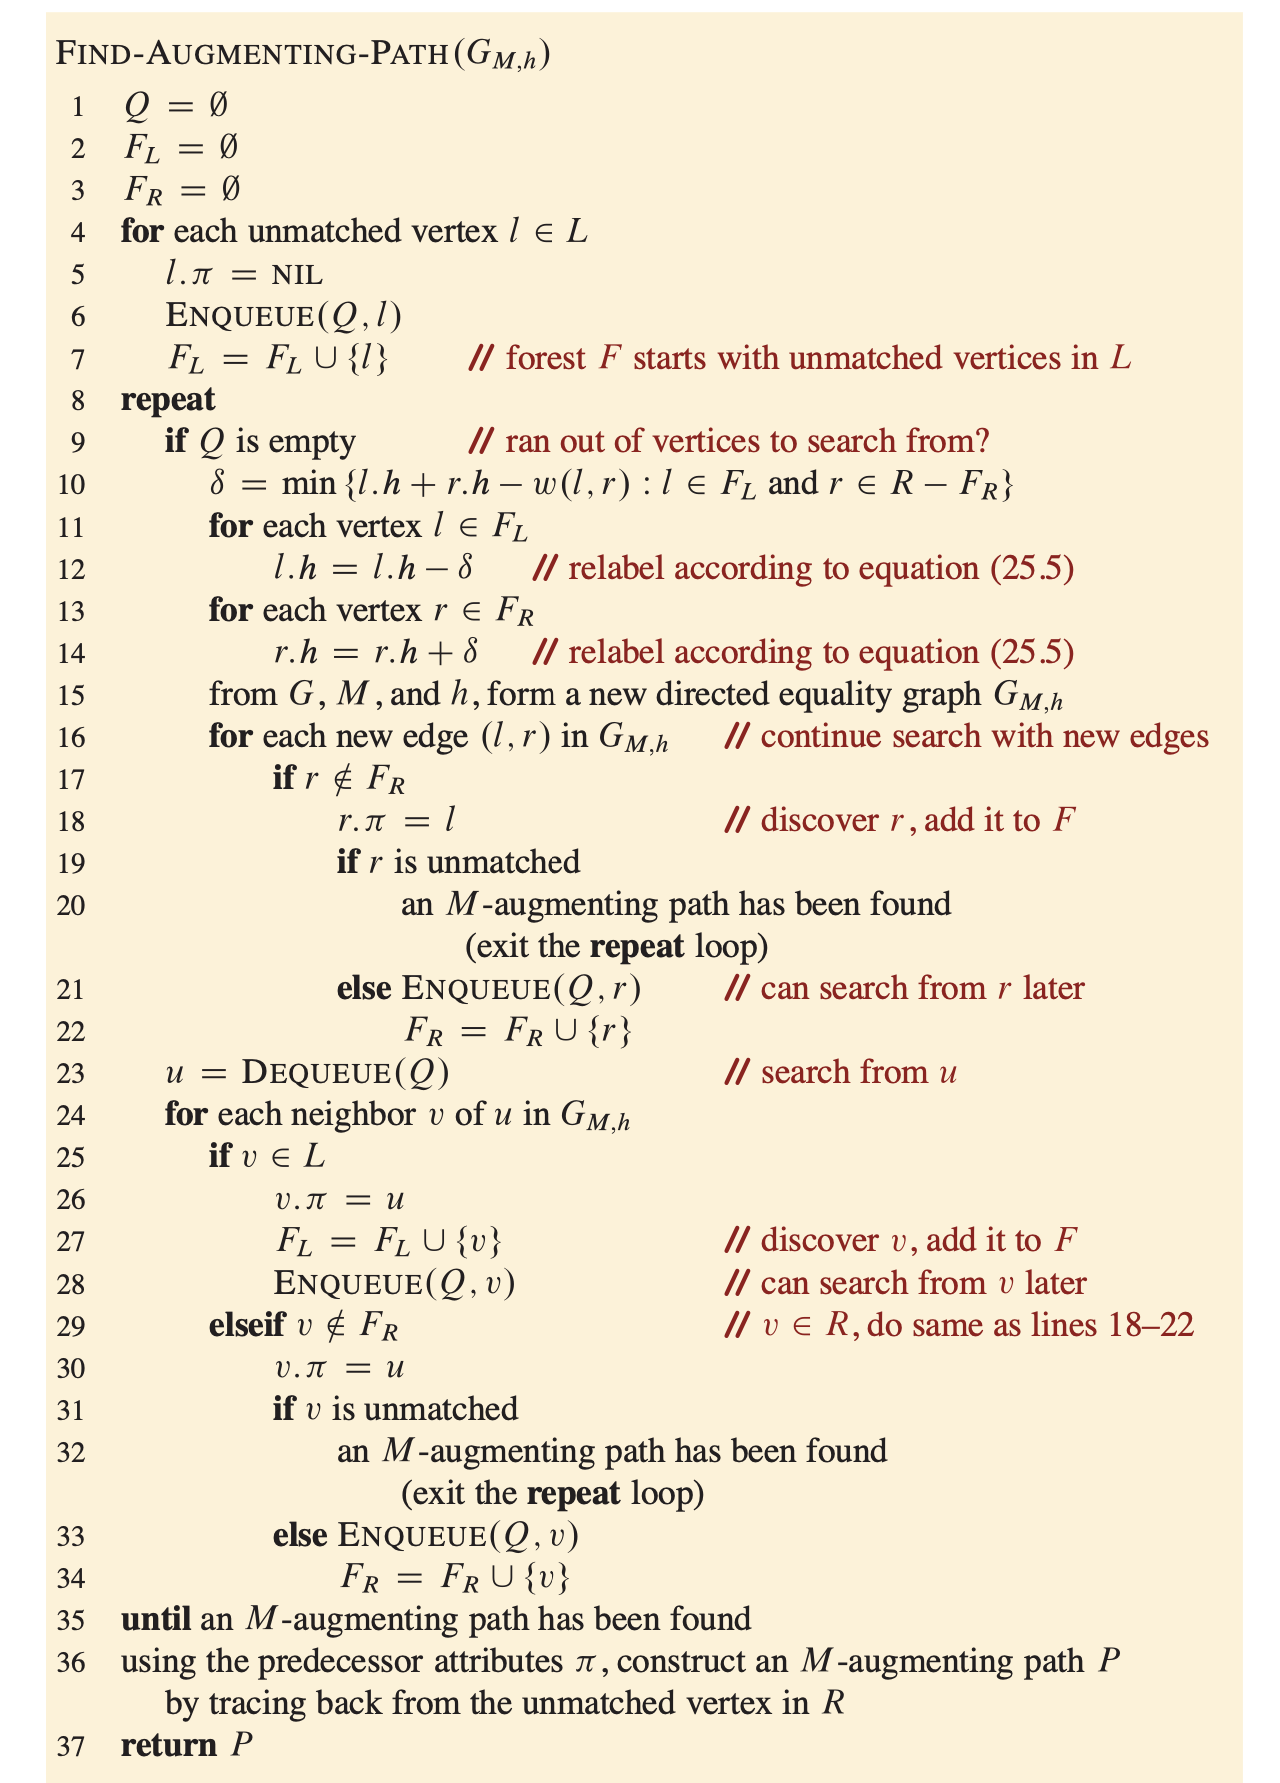
\includegraphics[width=0.8\textwidth]{Screenshot 2023-04-02 at 2.48.49 PM.png}
        \centering
        \caption{Find-Aumentative-Path\cite{4}}
    \end{figure}
    
    Note que: Un camino M-aumentativo en $G_{M,h}$ es también un camino M-aumentativo en $G_h$.Probemos esto \\
    Sea $C = \{ v_1,v_2,...,v_n\}$ un camino M-aumentativo en $M_{M,h}$\\
    $\forral$ arista dirigida $(v,u)\in M_{M,h}$ existe la arista (v,u) no dirigida en $M_h$ por como se construyen las aristas de $M_{M,h}$ (2)\\
    Luego $\forral  e \in C$ se puede construir un camino $C^{'}$ en $M_h$ tal que $e \in C^{'}$
    Luego $C^{'}$ nos brinda un cubrimiento que cubre al menos dos vértices mas que el emparejamiento M inicial en $M_h$. Por tanto $C^{'}$ es un camino M-aumentativo en $M_h$.\\
    Además al tener C y $C^{'}$ las mismas aristas entonces C y $C^{'}$ son iguales.\\
    \item ¿Qu\'e pasa si falla la búsqueda de un camino M-aumentativo?\\
    Respuesta: Es necesario actualizar el etiquetamiento de los vértices para a\~nadir al menos una arista.\\
    \subsubsection*{Argumentemos la respuesta anterior}
    Si aun no hemos llegado al emparejamiento perfecto y no encontramos caminos M-aumentativos en el grafo de igualdad dirigido $G_{M,h}$ es porque ya no tenemos vértices la cola por la que iniciar la búsqueda en el grafo y aun quedan vértice $r\in R$ si estar cubierto.\\
    Para resolver este problema es necesario actualizar el etiquetamiento factible, el algoritmo Húngaro lo hace de la siguiente manera :
    \begin{equation}
        v.h^{'} = \left\{\begin{array}{lcc}
                    v.h - \delta & si  ~v \in F_L \\
                    \\v.h + \delta & si ~v \in F_R \\
                    \\v.h & e.o.c & (v\in V - V_F)
                    
                    \end{array}
        \right.
    \end{equation}
    donde $\delta$ es diferencia mas peque\~na por la cual una arista incidente en $F_L$ deja de estar en el subgrafo de igualdad $G_h$, donde $F_L = L \cup V_F$ y $F_{R} = R \cap V_F$.\\
    el valor de $\delta$ se computa con la siguiente ecuación:\\
    \begin{equation}
        \delta = min \{l.h + r.h - w(l,r) : l \in F_L~and~ r\in R - F_R \}
    \end{equation}  
    
    Apoy\'andonos del \textbf{Lema 25.15} \cite{5}\footnote{ Let h be a feasible vertex labeling fof the complete bipartite grph G witch equality subgraph $G_h$, and let M be a martching for $G_h$ and F be a breadth-first forest being constructed for the directed equality subgraph $G_{M,h}$.Then, the labeling $h^{'}$ in equaition (3) is a feasible vertex labeling for G witch the following properties:\\
        \textbf{1} If (u,v) is an edge in the breadth-first orest F for $G_{M,h}$ then $(u,v) \in E_{M,h^{}'}$\\
        \textbf{2} If (l,r) belongs to the matching M for $G_{h}$,then $(l,r) \in E_{M,h^{'}}$\\
        \textbf{3} There exist vertices $l \in F_l$ and $r \in R - F_r$ such that $(l,r) \notin E_{M,h}$ but $(l,r) \in E_{M,h^{'}}$ 
    }
    podemos observar lo siguiente: al menos una nueva arista entra en el subgrafo dirigido de igualdad y cada arista que abandone dicho grafo no va a pertenecer ni a emparejamiento M ni al bosque F.\\
    Sea A el conjunto de las nuevas aristas que se a\~naden al subgrafo dirigido de igualdad $G_{M,h}$, $|A|\geq 1$\\
    Tomemos una arista cualquiera de A, llamémosle $(l_i,r_j)$, sabemos gracias al lema que esta arista va de $l_i \in L$ a $r_j\in R$,la manera de proceder con esta nueva informaci\'on ser\'a la siguiente: a\~nadimos esta arista al alg\'un \'arbol del bosque F(poniendo $l_i$ como predecesor de $r_i$) y continuamos realizando la búsqueda a partir de $r_i$, aqu\'i pueden pasar dos cosas.
    \begin{enumerate}
        \item $r_i$ no ha sido tomado, en este caso hemos encontrado un camino M-aumentativo
        \item $r_i$ se continua la búsqueda hasta encontrar $r\in R$ o hasta que ya no se pueda avanzar por ninguna arista.
    \end{enumerate}
    Dicho proceso proceso se hace con todas las aristas que pertenezcan a A.\\
    En caso de que la búsqueda de caminos M-aumentativos, se repite el proceso hasta encontrar un emparejamiento perfecto.\\
    Hasta equ\'i hemos demostrado la correctitud del algoritmo Húngaro . 
\end{enumerate}
\section*{Complejidad del algoritmo Húngaro}
 \begin{figure}[htb]
        \centering
        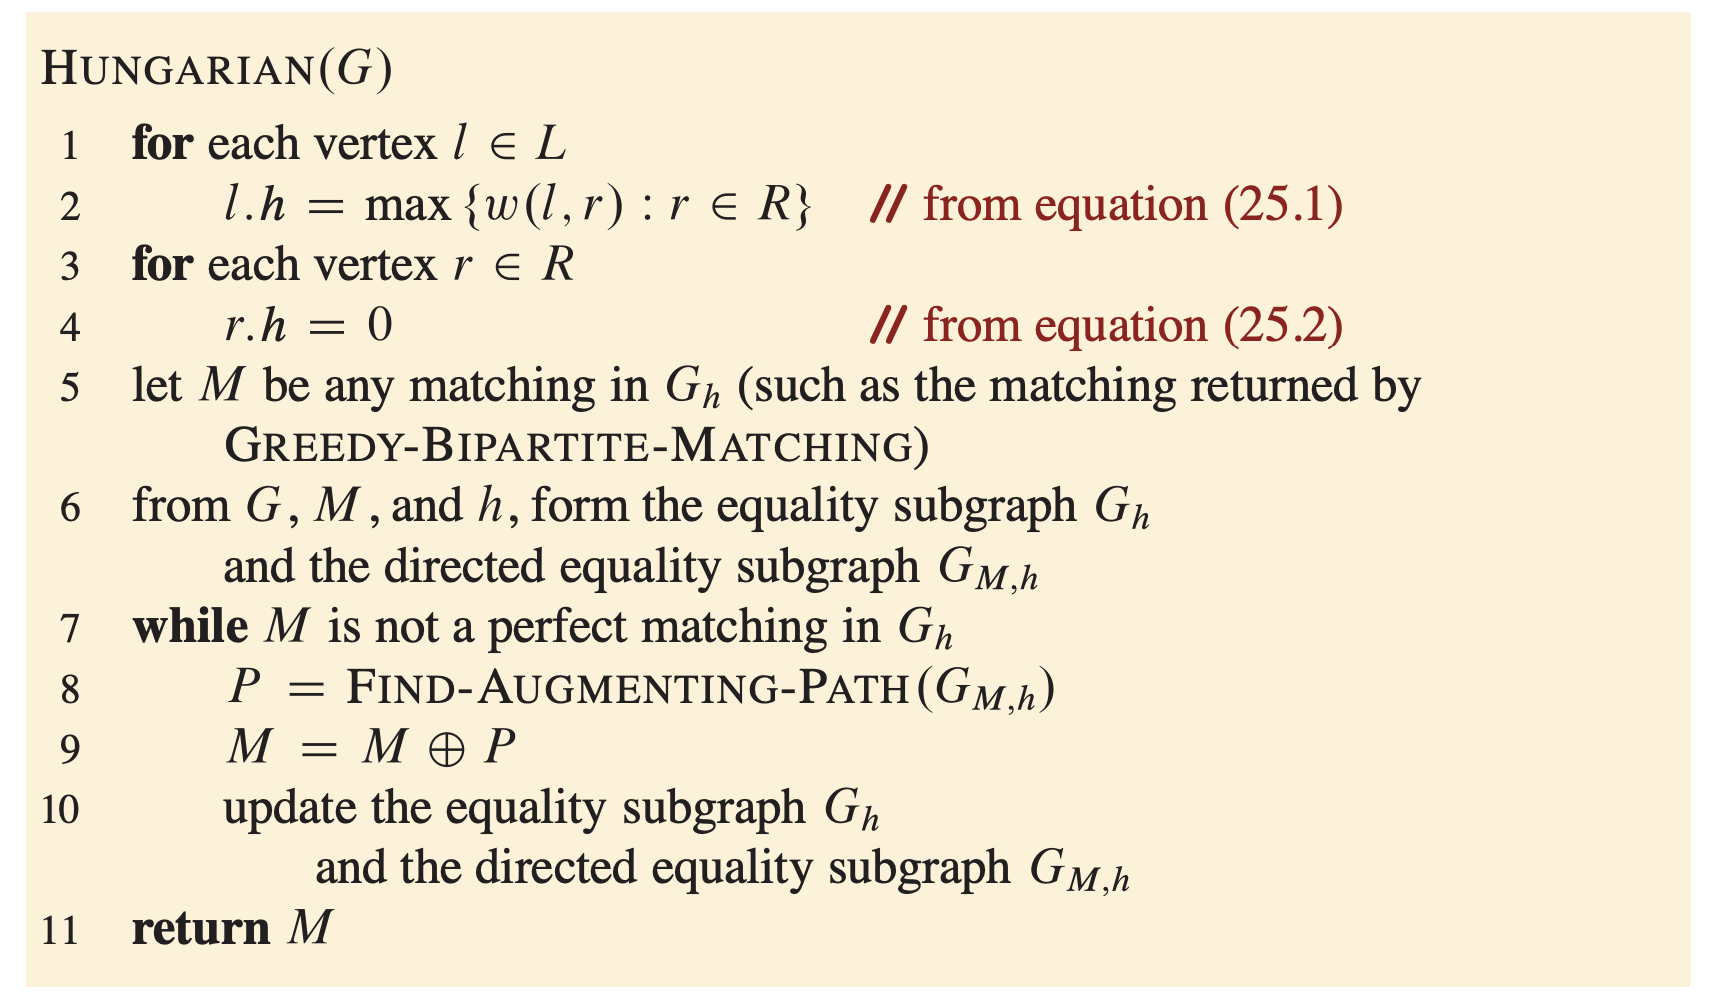
\includegraphics[width=0.8\textwidth]{Screenshot 2023-04-03 at 1.16.57 AM.png}
        \centering
        \caption{Hungarian\cite{6}}
    \end{figure}
En la \textbf{Fig 3} de la l\'inea 1-6 el algoritmo tiene una complejidad temporal de $O(n^2)$ ya que en la l\'inea de la 1-2  se halla el etiquetamiento  por defecto inicial  de los vértices $l\in L$ y para ello se recorren todos los vértices de L y a cada vértice $l\in L$ se recorren todas sus aristas(n-1, porque el grafo es bipartito completo y ponderado) y nos quedamos con la de mayor peso esto es $O(n^2)$ y de la l\'inea 3-4 se hace el etiquetamiento  por defecto inicial  de los vértices $r\in R$ esto es  $O(n)$.\\
El ciclo de la l\'inea 7-10 itera a lo sumo n veces incrementado en cada iteración el tama\~no del emparejamiento M en 1, comprobar la condición de ciclo($|M| \leq n$) es O(1), la l\'inea 9 tiene complejidad $O(n)$, esta l\'inea representa la acción de obtener un nuevo emparejamiento tras hacer diferencia simétrica con el emparejamiento actual de $G_h$ y el camino M-aumentativo obtenido con el algoritmo FIND-AUGMENTING-PATH, esto es $O(n)$ porque $|M|$ es a lo sumo n y la l\'inea 10 toma $O(n^2)$ porque para actualizar $G_h$ y $G_{M,h}$ es necesario recorrer las todas las aristas de G y $|E_G| = n^2$\\
Solo nos queda analizar dentro del ciclo la complejidad temporal de FIND-AUGMENTING-PATH, para ello nos apoyaremos en la \textbf{Fig 2} como hemos visto anteriormente esta función utiliza un BFS sobre $G_{M,h}$ para construir el bosque F, BFS tiene complejidad temporal $O(|V| + |E|) = O(n^2)$, además, en una llamada de esta función pueden ocurrir como máximo n pasos de crecimiento, ya que en cada paso de crecimiento esta garantizado al menos descubrir un vértice en R, en el ciclo de la l\'inea 16-22 itera máximo $n^2$ veces por cada llamado a  FIND-AUGMENTING-PATH. El cuello de botella esta en la l\'inea de la 10-15 que toma $O(n^2)$ porque actualiza el etiquetamiento de los vértices, por tanto FIND-AUGMENTING-PATH toma $O(n^3)$.
Luego el algoritmo Húngaro toma $O(n^4)$.
 
 \section*{Detalles de implementaci\'on }

 En la implementaci\'on de greedy bipartite matching se construye un matching que represente el subgrafo de igualdad
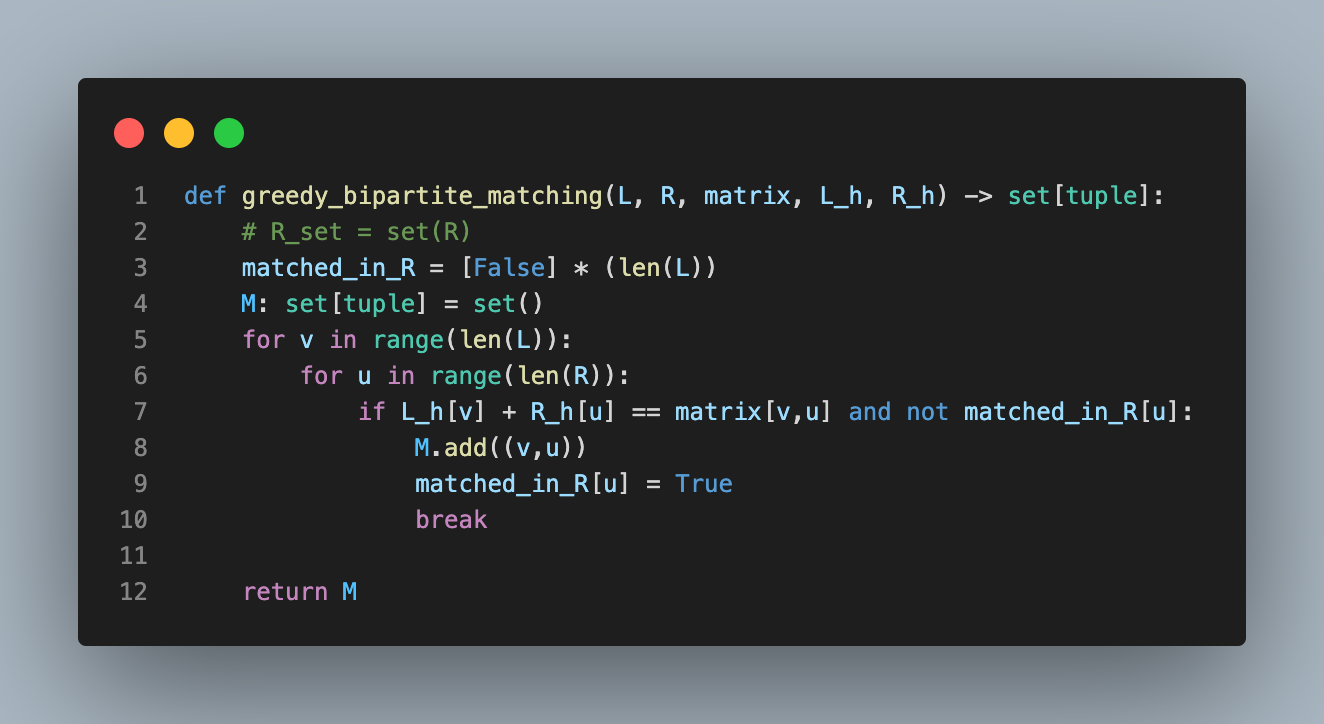
\includegraphics[width=0.8\textwidth]{1.png}
\\
La implementaci\'on se apoya en el ejercicio 25.3-5 para no tener que construir explicitamente el subgrafo dirigido de igualdad, podemos determinar si una arista pertenece al subgrafo dirigido de igualdad luego de actualizar el etiquetamiento. 
\begin{python}
for r in total_vertex:
    if r not in Fr and old_L_h[l] + old_R_h[r] > matrix[l,r] and L_h[l] + R_h[r] == matrix[l,r] and (l,r) not in M:


\end{python}
 \begin{figure}[htb]
        \centering
        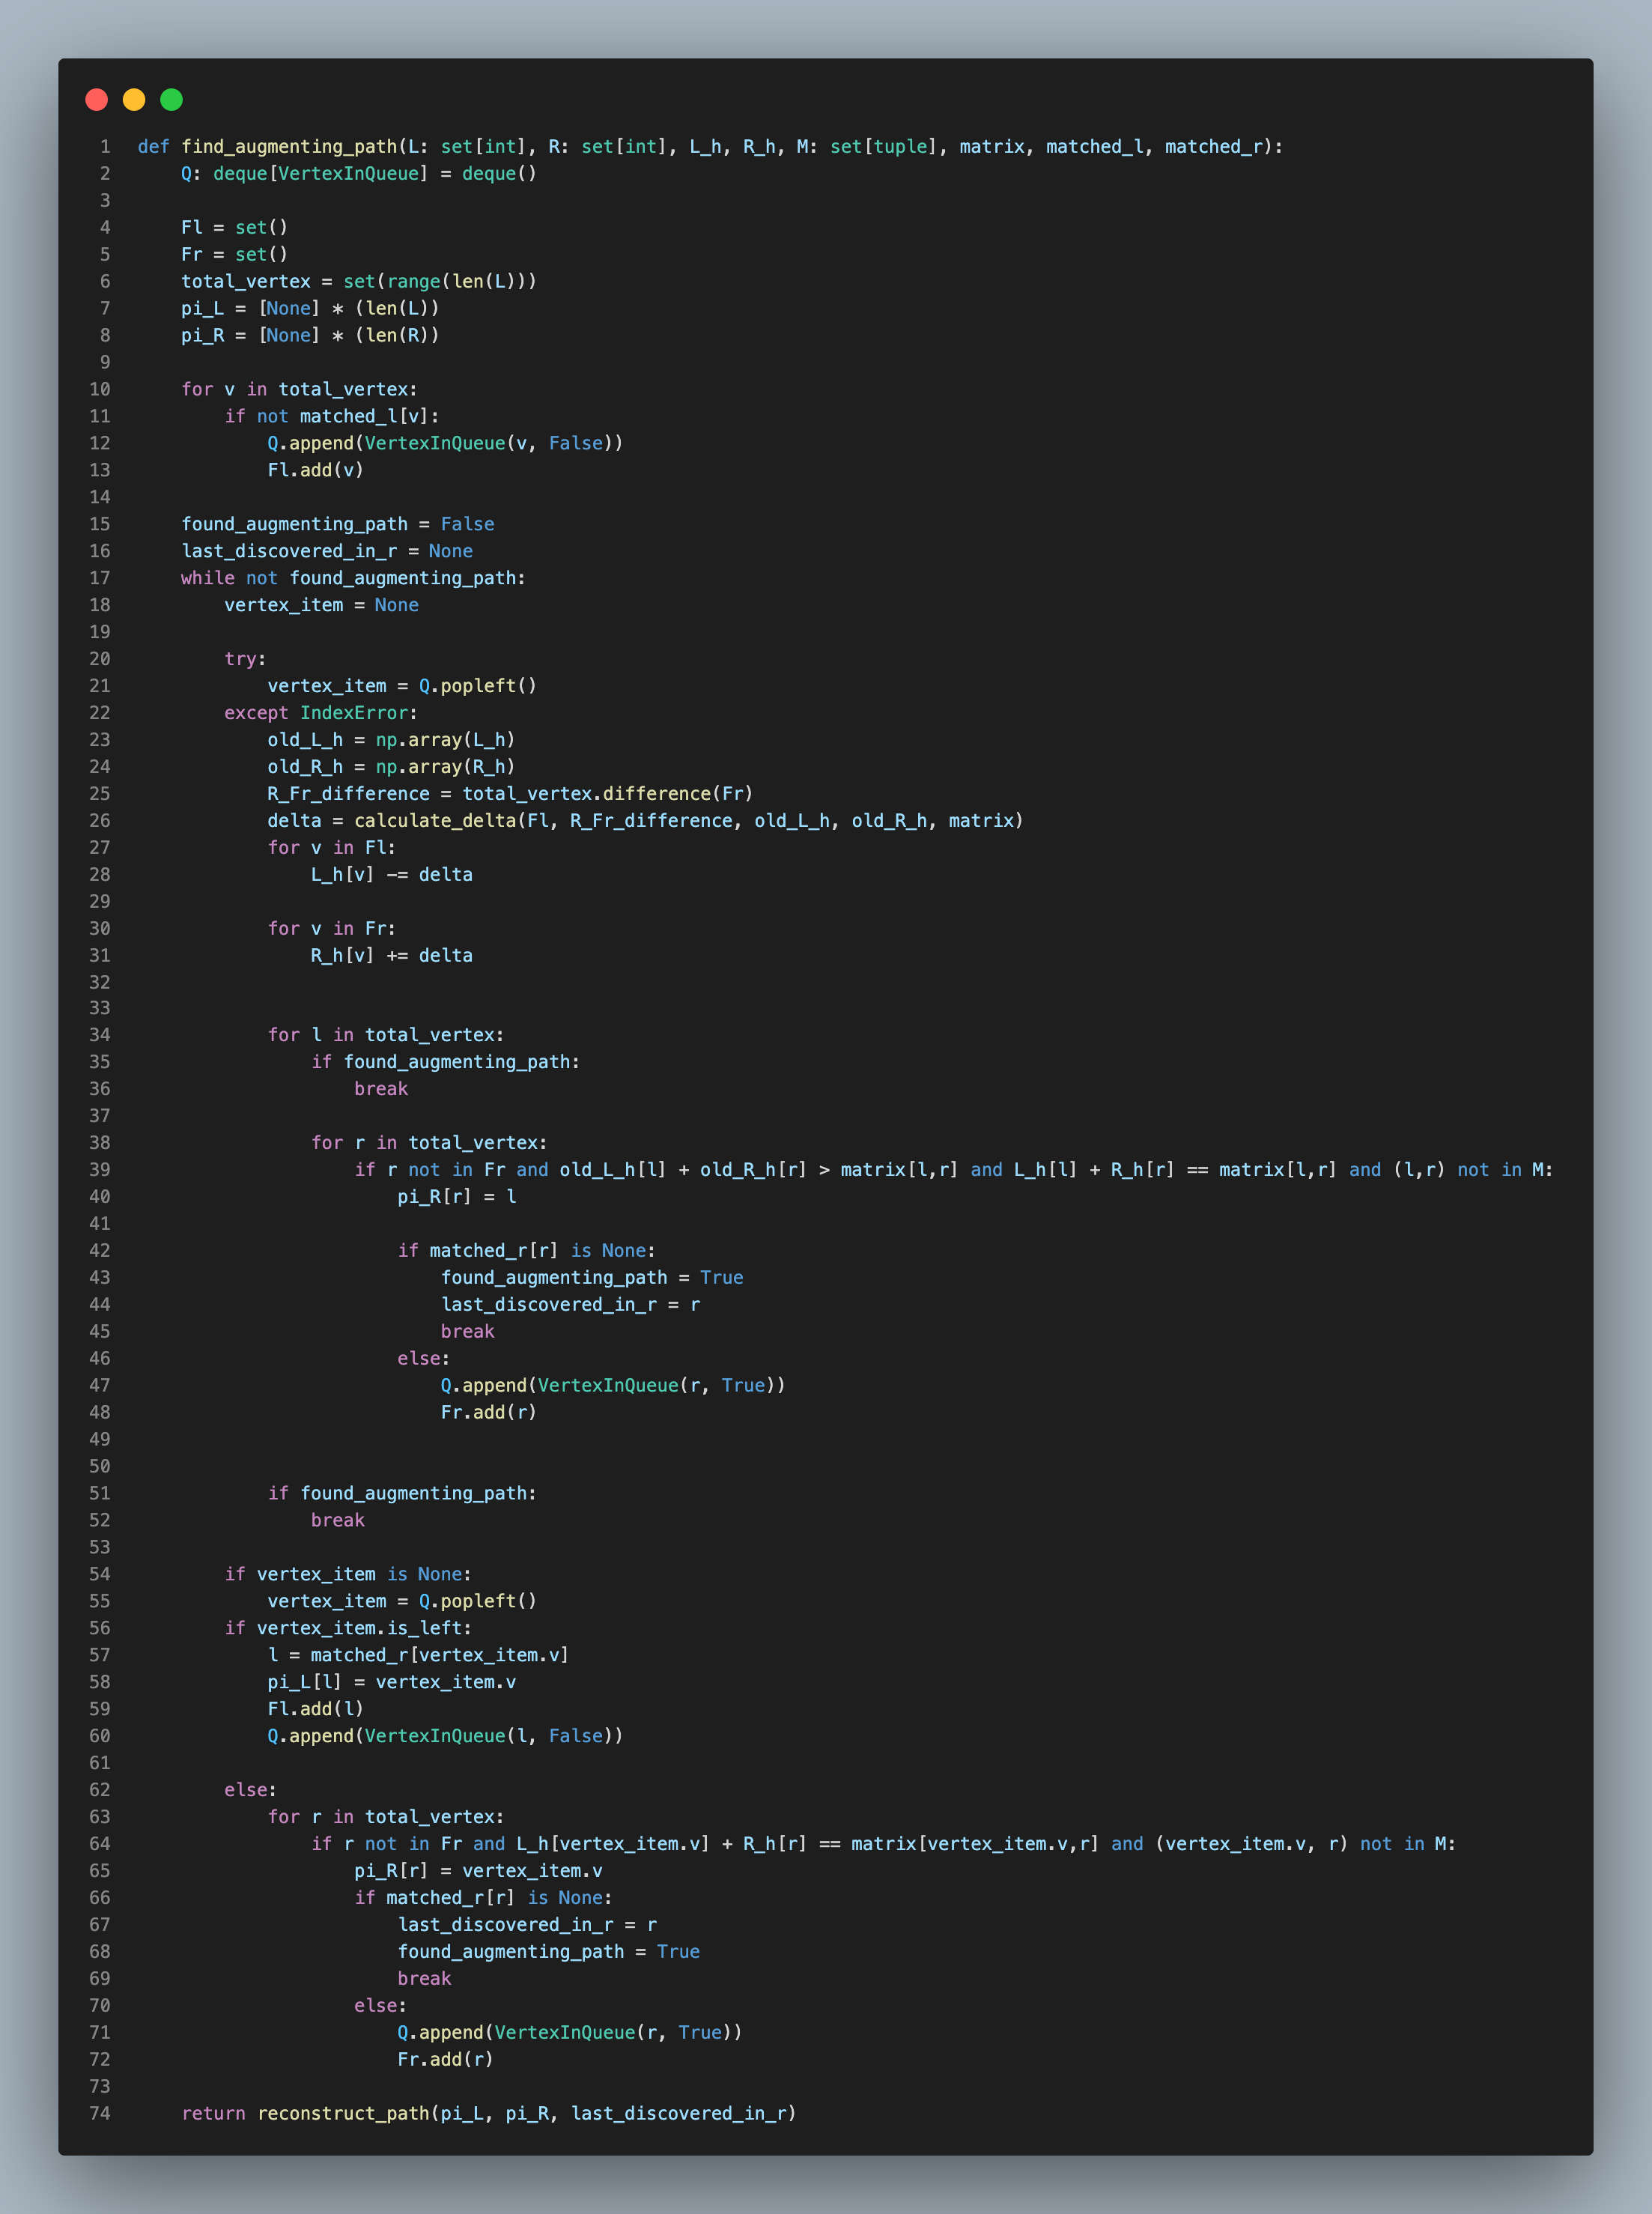
\includegraphics[width=0.6\textwidth]{2.png}
        \centering
    \end{figure}

     \begin{figure}[htb]
        \centering
        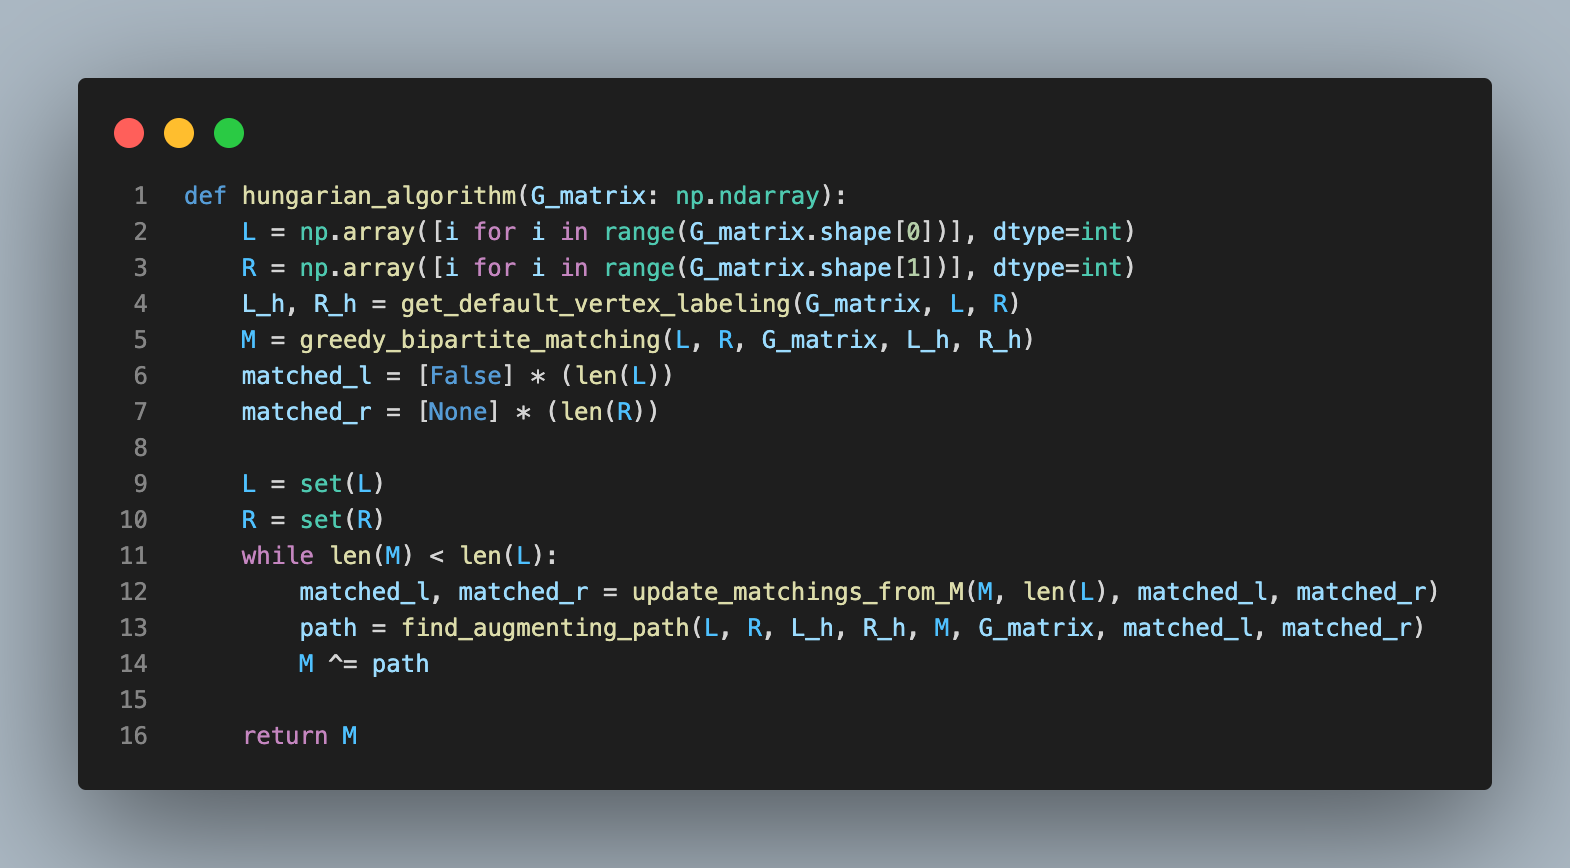
\includegraphics[width=0.6\textwidth]{3.png}
        \centering
    \end{figure}


 Se implement\'o una modificaci\'on del algoritmo para que tuviera una complejidad de $O(n^3)$ usando como gu\'ia el problema 25-2 del libro
Para cada v\'ertice r pertenece a R-Fr se define un atributo $r.\sigma$ donde:
$r.\sigma = min\{l.h + r.h - w(l,r): l~pertenece ~F_l\}$
r.o indica que tan cerca est\'a r de ser adyacente a alg\'un v\'ertice l pertenece a $F_l$ en el subgrafo dirigido de igualdad $G_{M,h} $.
\\
Inicialmente, antes de poner un v\'ertice en $F_l$ se hace $r.\sigma = \infty $ para todo r pertenece a R, luego de añadir los primeros v\'ertices a $F_l$ como en las lineas 4-7 del pseudocódigo de Find Augmenting Path, se calculan los $r.\sigma$ usando la definición anterior.\\
Con este atributo calcular delta se convierte en $O(n)$.
Dentro del ciclo while, hay 3 casos en los q se tienen q actualizar los $r.\sigma$, cuando se añade un vértice a $F_l$, cuando se añade un vértice a $F_r$ y cuando se actualizan los valores de delta.\\
En el primer caso es necesario recorrer todos los v\'ertices $R-F_r$ y comprobar si
$L\_h[l] + R\_h[r] - matrix[l,r] < r.\sigma$ \\
Esto es $O(n)$\\
En el segundo caso remover el vértice del conjunto que mantiene $R-F_r$\\
En el tercer caso solo interesa tener el cambio de los l.h ya q los r.h que cambian pertenecen a $F_r$, para esto se recorren todos los $r.\sigma$ y se les resta delta a sus valores, esto es $O(n)$, con este paso si una nueva arista pertenecerá a $G_{M,h}$ en el momento que un $r.\sigma$ se haga 0.\\

Luego, podemos concluir que con esta modificaci\'on Find-Augmenting-Path es $O(n^2)$ \\

\begin{figure}[htb]
        \centering
        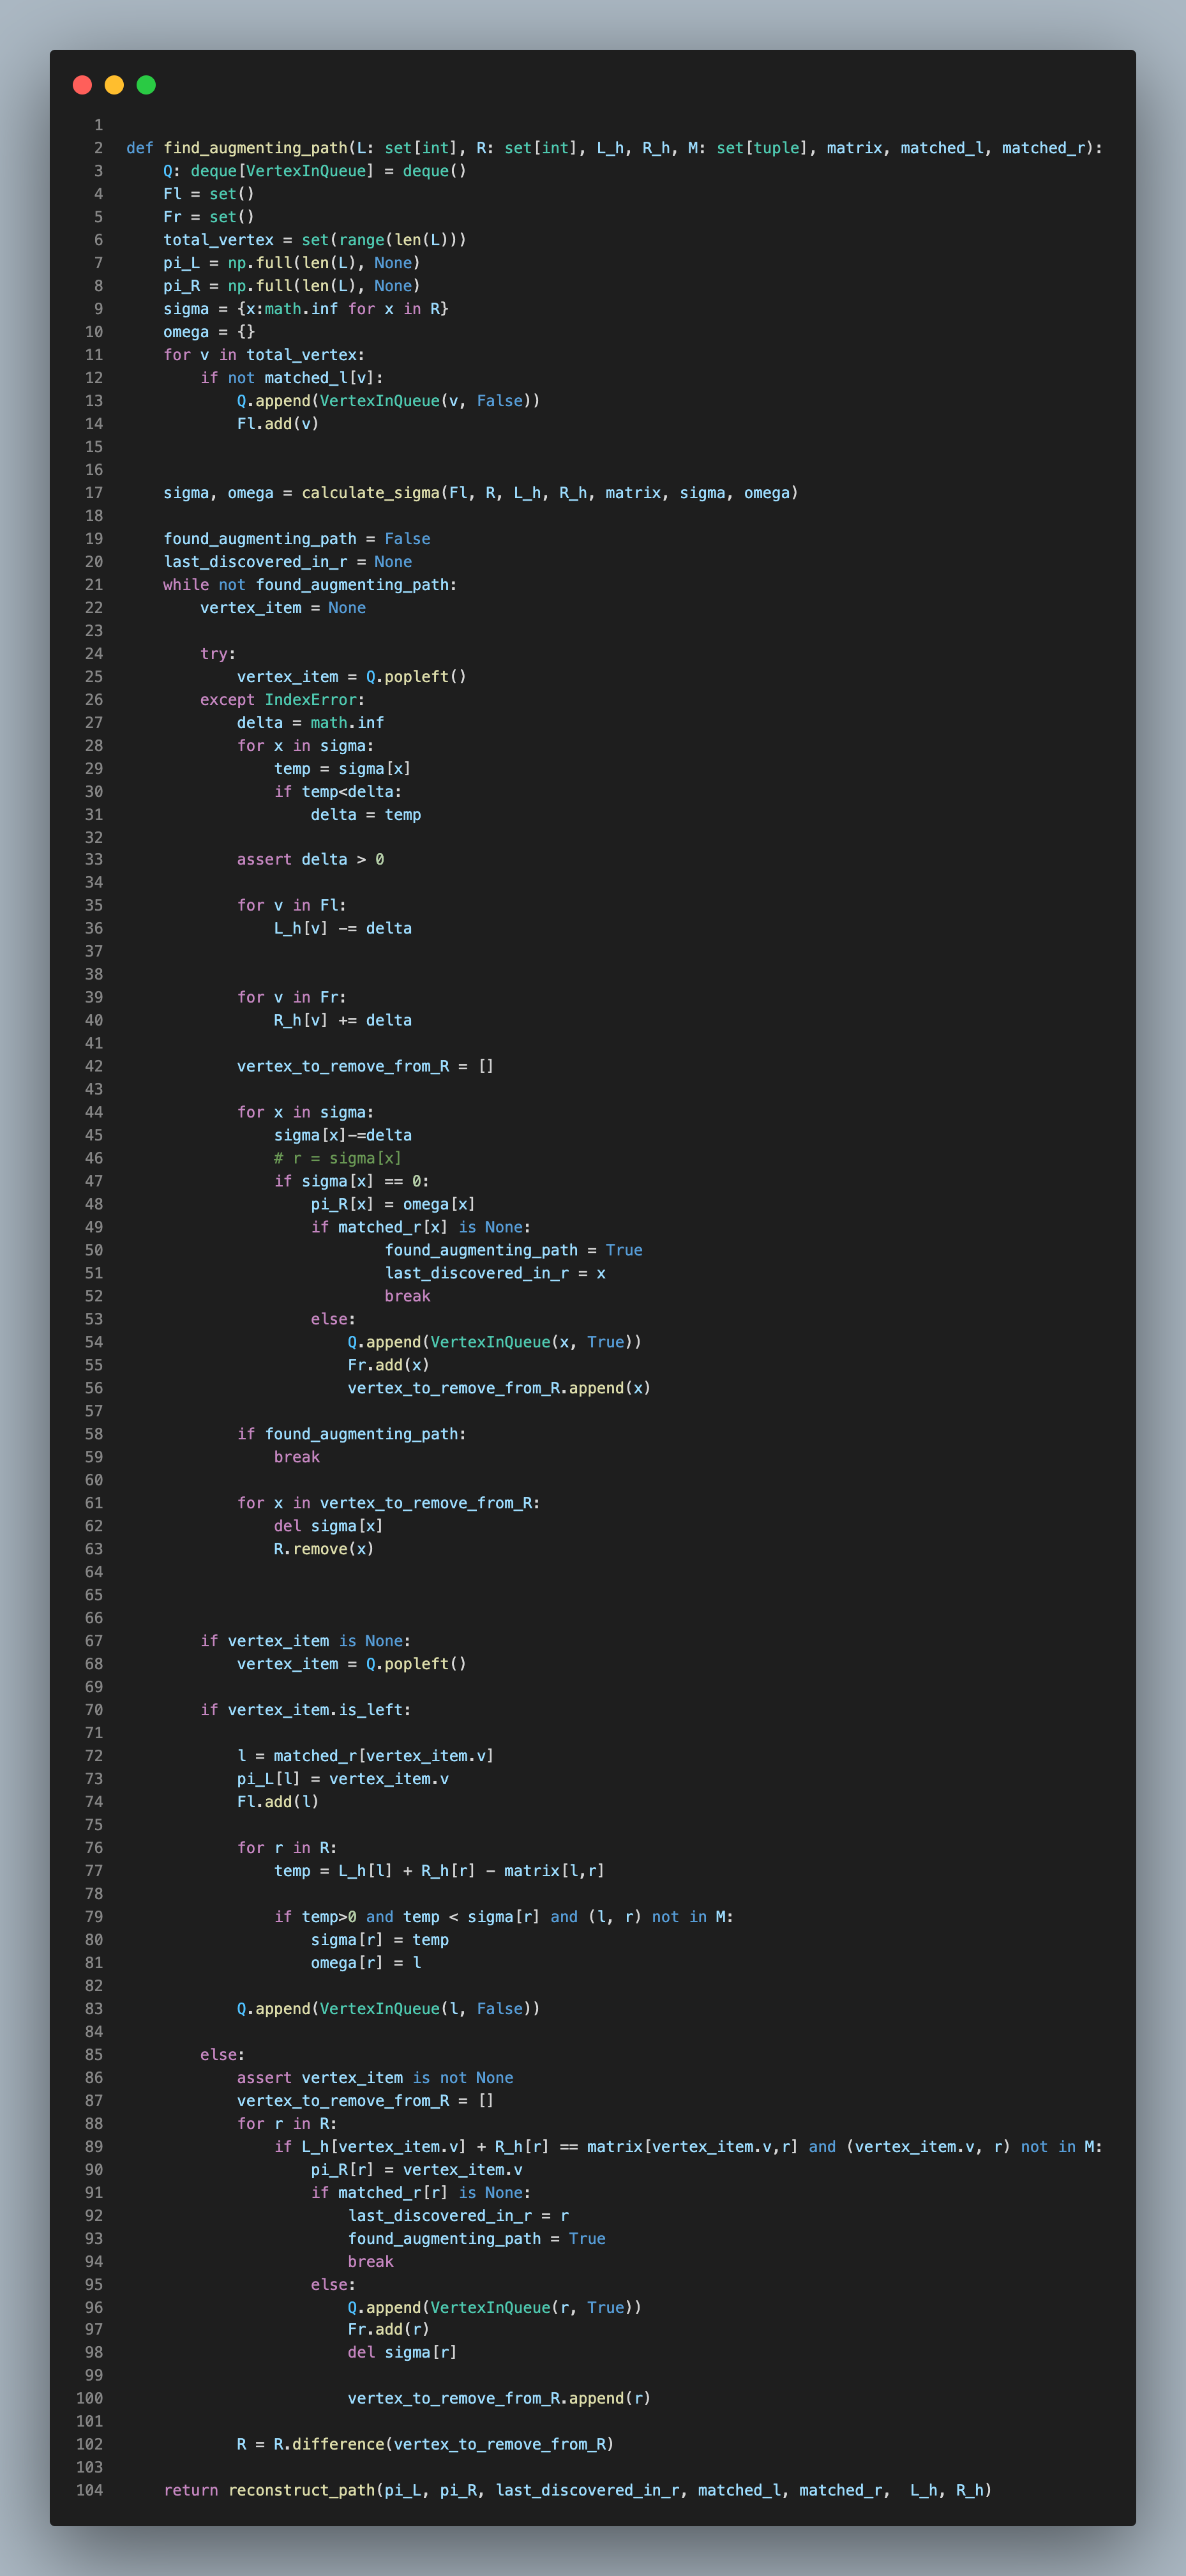
\includegraphics[width=0.5\textwidth]{codel.png}
        \centering
    \end{figure}
 
 
\begin{thebibliography}{99}
\bibitem{1} thomas-h-cormen-introduction-to-algorithms-4th-edition parte VI cap
 cap 25.3.
 \bibitem{2} Theorem 25.14, Parte VI cap25.3 de thomas-h-cormen-introduction-to-algorithms-4th-edition.
 \bibitem{3} Parte VI cap25.3 p\'agina 726 de thomas-h-cormen-introduction-to-algorithms-4th-edition.
\bibitem{4} Parte VI cap25.3 p\'agina 738 de thomas-h-cormen-introduction-to-algorithms-4th-edition.
\bibitem{5} Parte VI cap25.3 p\'agina 731 Lemma 25.15 de thomas-h-cormen-introduction-to-algorithms-4th-edition.
\bibitem{6} Parte VI cap25.3 p\'agina 737 de thomas-h-cormen-introduction-to-algorithms-4th-edition.
\end{thebibliography}

\end{document}


